%class
	\documentclass{beamer}

%template
	\usetheme{HannoverSalman}
	\setbeamertemplate{navigation symbols}{}
	%\setbeamertemplate{footline}{\centering{\insertframenumber/\insertpresentationendpage}}
	%\setbeamertemplate{footline}{\hspace*{.5cm}\scriptsize{\hfill\insertframenumber\hspace*{.5cm}}} 


%packages
	\usepackage{amsmath, amssymb, graphicx,cancel}
	\usepackage[absolute,overlay]{textpos}
	\usepackage{subfigure}
	\usepackage{caption}\captionsetup{labelformat=empty,labelsep=none}
	\usepackage{geometry}
	\geometry{verbose}
	\usepackage{color}
	\usepackage{xmpmulti}
	\usepackage[3D]{movie15}
	\usepackage{hyperref}
%	\usepackage{bookmark}
	\usepackage[open,openlevel=4,atend]{bookmark}
	%\bookmarksetup{color=blue}
	\usepackage{multirow}
	\usepackage[style=numeric,defernumbers, authoryear]{biblatex}
	%\usepackage[square,sort]{natbib}
	%\usepackage{fancyhdr}%\pagestyle{fancy} 

	
	\hypersetup{bookmarksdepth = 4}


%citations files
	\bibliography{MyCitations}

%logoCSIPCPL
    \setlength{\TPHorizModule}{1mm}
    \setlength{\TPVertModule}{1mm}
    \newcommand{\logoCSIPCPL}
    {
    	\begin{textblock}{1}(100,2) %(100,85)  for bottom
    		
\includegraphics[width=1.5cm]{figs/logo_CSIP}
    	\end{textblock}
    	
	\begin{textblock}{1}(117,1) %(117,85)  for bottom
    		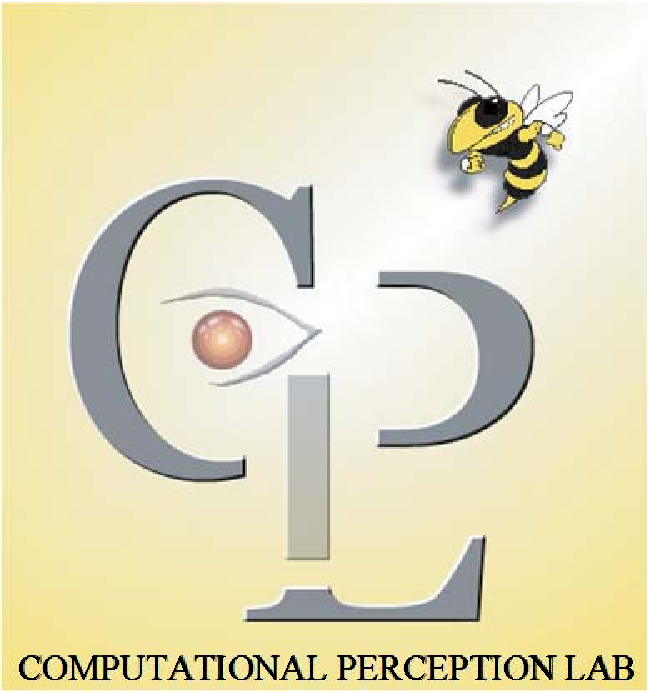
\includegraphics[width=1.0cm]{figs/logo_CPL}
    	\end{textblock} 
    }

%logo evolution
    \newcommand{\logoEvolution}
    {    	
	\begin{textblock}{1}(110,1) %(117,85)  for bottom
    		\includegraphics[width=0.65in]{figs/logo_evolution.pdf}
    	\end{textblock} 
    }

%logo Qualcomm
    \newcommand{\logoQualcomm}
    {
    	\begin{textblock}{1}(110,2) %(100,85)  for bottom
    		\includegraphics[width=1.5cm]{figs/logo_qualcomm.jpg}
    	\end{textblock}
    }
%logo Qualcomm (long)
    \newcommand{\logoQualcommllong}
    {
    	\begin{textblock}{1}(0,0) 
    		\includegraphics[width=1.25in]{figs/logo_qualcomm_long.jpg}
    	\end{textblock}
    }

%logo Tech Tower
    \newcommand{\logoTechTower}
    {
    	\begin{textblock}{1}(0,0) 
    		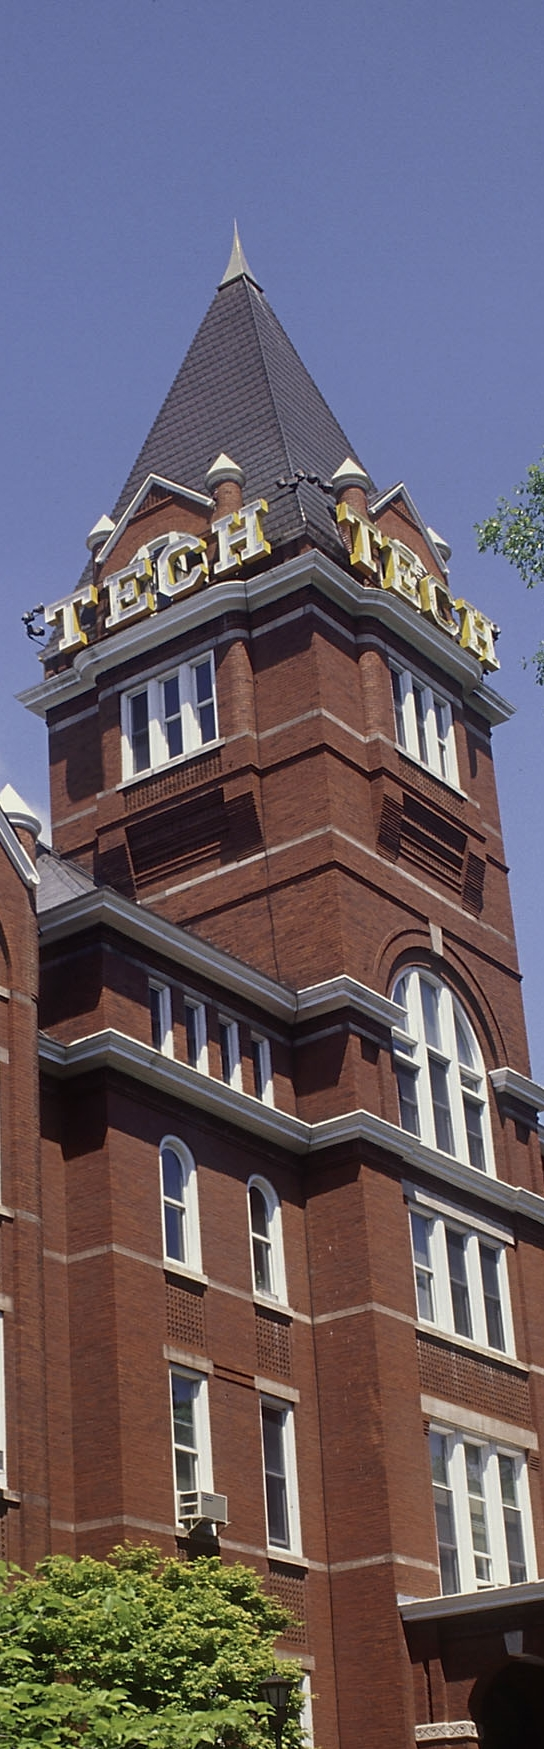
\includegraphics[width=1.25in]{figs/logo_TechTower.jpg}
    	\end{textblock}
    }

%logo tree
    \newcommand{\logoTree}
    {
    	\begin{textblock}{1}(0,0) 
    		\includegraphics[width=1.25in]{figs/logo_tree.jpg}
    	\end{textblock}
    }
%page numbers
    \newcommand{\mypagenum}
    {
    	\begin{textblock}{1}(1,94) 
		{\tiny \color[rgb]{0.2,0.2,1}\insertframenumber} %\insertframenumber,\insertpresentationendpage, \inserttotalframenumber
    	\end{textblock}
    }
%my footnote citation
	\newcommand{\myFootnoteCitation}[2]
	{
		\footnote{\tiny \citeauthor{#1}, \emph{#2}, \citeyear{#1}.}  %\citeauthor{#1}, \citetitle{#1}, #2 \citeyear{#1}.
	}
%my refer to citation
	\newcommand{\mycite}[1]
	{
		\emph{\citeauthor{#1} (\citeyear{#1})}
	}
%my footnote website citation
	\newcommand{\myFootnoteWebsiteCitation}[1]
	{
		\footnote{\tiny \citeauthor{#1}}
	}

\let\thefootnote\relax\footnotetext{Footnotetext without footnote mark}


%section underline
%\newcommand{\tmpsection}[1]{}
%\let\tmpsection=\section
%\renewcommand{\section}[1]{\tmpsection{\underline{#1}}}



%commands
	\newcommand{\likelihood}{p(Z_k| x_k) }						%likelihood
	\newcommand{\prior}{p(x_k)  } 								%prior
	\newcommand{\posterior} {p(x_k| Z_k)}						%posterior
	\newcommand{\prediction} {p(x_k| Z_{k-1})}					%prediction
	\newcommand{\update} {p(x_k|Z_k)}							%update
	\newcommand{\observations} {p(Z_k)}						%observations
	\newcommand{\prevobservations} {p(Z_{k-1})}				%previous observations
	\newcommand{\dxpk} {dx_{k-1}}							%dx_{k-1}
	\newcommand{\ChapKolm}{\int{p(x_k| x_{k-1})p(x_{k-1}|Z_{k-1})} \dxpk} %Chapman Kolmogorov

	%algorithm specific: JPDAF
	\newcommand{\likelihoodJPDAF}{p(Z_k| \chi, m, Z_{k-1}) }		%1. likelihood
	\newcommand{\priorJPDAF}{p(\chi|m, Z^{k-1}} 				%2. prior	
	\newcommand{\observationsJPDAF} {p(Z_k}					%3. observations
	\newcommand{\posteriorJPDAF} {p(\chi| Z_k)}					%4. posterior

%environments
	\newenvironment{changemargin}[2]
	{
	  	\begin{list}{}
		{
			\setlength{\topsep}{0pt}%
			\setlength{\leftmargin}{#1}%
			\setlength{\rightmargin}{#2}%
			\setlength{\listparindent}{\parindent}%
			\setlength{\itemindent}{\parindent}%
			\setlength{\parsep}{\parskip}%
		}
	  	\item[]
		}
		{\end{list}
	}
%figures

%colors
\definecolor{darkgreen}{rgb}{0,0.5,0}

%personal details
	\author{Salman Aslam}
	\institute{Advisor, Dr Christopher Barnes (ECE)\\Co-advisor, Dr Aaron Bobick (CoC)\\Georgia Institute of Technology}
	\date{}

\begin{document}
\definecolor{darkgreen}{rgb}{0,0.5,0}
\newcommand{\Ntrg}{\big[N_{t=1, m=1} + \lambda \big] + \big[N_{t=1, m=2} + \lambda \big] + \ldots + \big[N_{t=1, m=M} + \lambda \big]}
\newcommand{\jointcnt}{\sum\limits_{n_{trg}=1}^{N_{trg}}I(X_t=x_t, X_{t-1}=x_{t-1})}
\newcommand{\singlecnt}{\sum\limits_{n_{trg}=1}^{N_{trg}}I(X_{t-1}=x_{t-1})}
\newcommand{\singlep}{p(X_{t-1}=x_{t-1})}
\newcommand{\singlepone}{p(X_{t-1}=1)}
\newcommand{\singleptwo}{p(X_{t-1}=2)}
\newcommand{\singlepM}{p(X_{t-1}=M)}
\newcommand{\condp}{p(X_t=x_t | X_{t-1}=x_{t-1})}
\newcommand{\jointp}{p(X_t=x_t, X_{t-1}=x_{t-1})}
\newcommand{\KmeansOuterSum}{\sum\limits_{k=1}^K}
\newcommand{\KmeansInnerSum}{\sum\limits_{{i=1 \atop x_i \in \mathcal{K}_k}}^N}
\newcommand{\KmeansSum}{\KmeansOuterSum \KmeansInnerSum}
\newcommand{\RVQInnerSum}{\sum\limits_{{i=1 \atop g_i \mapsto m_{\tau, s}}}^N}
\newcommand{\RVQOuterSum}{\sum_{s=1}^S}
\newcommand{\RVQsum}{\KmeansOuterSum \sum\limits_{{i=1 \atop g_i \in \mathcal{K}_k}}^N}
\newcommand{\KmeansInner}{{(x_i - \mu_k)}^2}
\newcommand{\RVQinner}{            {(x_i  - \hat{\mu}^{(k)})}^2}
\newcommand{\RVQinneralternate}{{(g_i - m_\tau^{(k)})}^2}
\newcommand{\RVQinneralternatealternate}{{(g_i - m_{\tau, s})}^2}
\newcommand{\KmeansError}{\KmeansSum \KmeansInner}
\newcommand{\RVQerror}     {\KmeansSum \RVQinner}
\newcommand{\RVQerroralternate}{\RVQsum \RVQinneralternate}
\newcommand{\RVQunit}{x_i -\bigg(\sum_{t=1}^Tm^{(k)}_t\bigg)}
\newcommand{\RVQequivalentCodevector}{\sum_{t=1 }^Tm^{(k)}_t}
\newcommand{\RVQequivalentCodevectorBroken}{\sum_{t=1 \atop t \neq \tau}^Tm^{(k)}_t+ m^{(k)}_\tau}
\newcommand{\RVQmultipleKmeans}{x_i -\bigg(\RVQequivalentCodevectorBroken\bigg)}
\newcommand{\RVQmultipleKmeansone}{x_i -\sum_{t=2}^Tm^{(k)}_t+ m^{(k)}_1\bigg)}
\newcommand{\RVQmultipleKmeansonealternate}{\bigg(x_i -\sum_{t=1 \atop t \neq \tau}^Tm^{(k)}_t\bigg) - m^{(k)}_\tau}
\newcommand{\RVQmultipleKmeanstwo}{x_i -\bigg(\sum_{t=1 \atop t \neq 2}^Tm^{(k)}_t+ m^{(k)}_2\bigg)}
\newcommand{\RVQmultipleKmeansT}{x_i -\bigg(\sum_{t=1}^{T-1}m^{(k)}_t+ m^{(k)}_2\bigg)}
\newcommand{\EucMatrix}
{
\left[
\begin{array}{lll}
r_{11} & r_{12} & t_x \\ 
r_{21} & r_{22} & t_y \\ 
0 & 0 & 1 \\ 
\end{array}
\right]
}	

\newcommand{\SimMatrix}
{
\left[
\begin{array}{lll}
sr_{11} & sr_{12} & t_x \\ 
sr_{21} & sr_{22} & t_y \\
0 & 0 & 1 \\ 
\end{array}
\right]
}

\newcommand{\AffMatrix}
{
\left[
\begin{array}{lll}
a &b & t_x \\ 
c & d & t_y \\
0 & 0 & 1 \\
\end{array}
\right]
}

\newcommand{\ProjMatrix}
{
\left[
\begin{array}{lll}
h_{11} & h_{12} & h_{13} \\ 
h_{21} & h_{22} & h_{23} \\ 
h_{31} & h_{32} & h_{33} \\ 
\end{array}
\right]
}

\newcommand{\RotMatrixTheta}
{
\left[
\begin{array}{rr}
\cos(\theta) & -\sin(\theta) \\ 
\sin(\theta) & \cos(\theta) \\ 
\end{array}
\right]
}

\newcommand{\RotMatrixPhi}
{
\left[
\begin{array}{rr}
\cos(\phi) & -\sin(\phi) \\ 
\sin(\phi) & \cos(\phi) \\ 
\end{array}
\right]
}

\newcommand{\RotMatrixminusPhi}
{
\left[
\begin{array}{rr}
\cos(-\phi) & -\sin(-\phi) \\ 
\sin(-\phi) & \cos(-\phi) \\ 
\end{array}
\right]
}


\newcommand{\EigenvalueMatrix}
{
\left[
\begin{array}{cc}
\lambda_1 & 0\\
0 & \lambda_2
\end{array}
\right]
}

\newcommand{\bigMatrix}
{
s \left[
\begin{array}{cc}
 (r)(a) + b &  (r)(d) - c \\
 (r)(c) - d &  (r)(b) + a
\end{array}
\right]
}


\newcommand{\bigMatrixTwo}
{
\left[
\begin{array}{cc}
(\lambda_2) p + (\lambda_1) q & (\lambda_2) s  - (\lambda_1) r \\
(\lambda_2) r  - (\lambda_1) s & (\lambda_2) q + (\lambda_1) p
\end{array}
\right]
}
\newcommand{\dr}{(\mathbf{x}_i-\boldsymbol\mu_k)^T(\mathbf{x}_i-\boldsymbol\mu_k) + \lambda({Q_{\textrm{max}}-Q_i})}





\begin{frame}[plain]
\frametitle{Linear Gaussian Model\footnote{Roweis 1999, Tipping, 1999}}
\framesubtitle{Unifying PCA, PPCA, FA, and VQ.}
\logoCSIPCPL\mypagenum

\begin{changemargin}{-1.3in}{0in}
\begin{equation}
\begin{array}{llllllllllllll}
\mathbf{x}_{t+1} &=  \mathbf{A}\mathbf{x}_{t} +  \mathbf{w}_t   & & & \mathbf{w}_t \sim \mathcal{N}(0, \mathbf{Q})\\
\mathbf{y}_t 		 &=  \mathbf{C}\mathbf{x}_{t} +  \mathbf{v}_t    & & & \mathbf{v}_t \sim \mathcal{N}(0, \mathbf{R})
\end{array}
\label{LGM}
\end{equation}
\small
\begin{table}[t]
\centering
\begin{tabular}{| c | c | c | c | c |}\hline
 				 	&\textbf{A}	 	&	\textbf{C}  									& \textbf{Q} 	&  \textbf{R}                                                                		\\\hline
\textbf{PCA} 	&\textbf{0}		&	principal eigenvectors of $\boldsymbol\Sigma$	& \textbf{I}  	&  $\lim\limits_{\sigma^2 \rightarrow 0} \sigma^2\mathbf{I}$ 	\\\hline
\textbf{PPCA} &\textbf{0}		& 	scaled principal eigenvectors of $\boldsymbol\Sigma$	& \textbf{I}	&										      $\sigma^2 \mathbf{I}$	 \\\hline
\textbf{FA}   	&\textbf{0}		&	-												& \textbf{I} 	&  diagonal matrix 																\\\hline
\textbf{VQ}	 	&\textbf{0} 	&	cluster means								& \textbf{I}	& 	-																					\\\hline
\end{tabular}
\label{table:LGM_unifying}
\end{table}
\begin{equation}
\begin{array}{llllllllllllll}
\mathbf{x} &= \mathbf{WTA}(\mathbf{w}) 						& & & \mathbf{w} &\sim \mathcal{N}(\mathbf{\boldsymbol\mu}, \mathbf{Q})\\
\mathbf{y} &=  \mathbf{C}\mathbf{x} +  \mathbf{v} 		& & & \mathbf{v} & \sim \mathcal{N}(0, \mathbf{R})
\end{array}
\label{LGM2}
\end{equation}
\end{changemargin}
\end{frame}




\begin{frame}
\scriptsize
\begin{table}[htp]
\begin{tabular}{| c ||c | c| c|}
\hline
											&ESVQ						&TSVQ																&RVQ								\\ 
\hline
\# data points								&$N$						&same																&same								\\ 
\hline
Vertical dimension, $T$					&-							&depth																&\# stages							\\
Horizontal dimension, $M$					&-							&breadth															&\# templates						\\
Encoding indeces							&-							&path map	(T-tuple)												&XDR (T-tuple)						\\ 
\hline
Input dimension							&$D$						&same																&same								\\
Rate, $r$ (bits/vector component)			&$(\log_2K)/D$			&same																&same								\\ 
\hline
\# non-terminal codevectors, $N_{ntc}$	&0							&$1+M+M^2+ \ldots + M^{T-1}=\frac{M^T-1}{M-1}$			&$MT$								\\
\# terminal codevectors, $K$				&$2^{rD}$					&$2^{rD}=M^T$													&same as TSVQ					\\
\hline
computations: search ops/stage			&1 stage, $O(2^{rD})$	&$M$																&same as TSVQ					\\
computations: search complexity 			&$O(2^{rD})$				&O($MT$)															&same  as TSVQ					\\ 
memory 									&$2^{rD}$					&$MN_{ntc} = M\frac{M^T-1}{M-1}\approx\frac{M}{M-1}M^T$ &$MT$								\\ 
\hline
\# Input data at stage $t$					&1 stage, $N$				&$\frac{N}{M^t}$													&$N$								\\
\hline
\end{tabular}
\caption{Comparison of ESVQ, TSVQ and RVQ}
\label{tab:comparison_ESVQ_TSVQ_RVQ}
\end{table}
\end{frame}

%####################################################################################################
%####################################################################################################
%\bibliographystyle{ieee}
%\bibliography{c:/salman/work/writing/MyCitations}
\end{document}
%####################################################################################################

%####################################################################################################
